% !TeX encoding = UTF-8
% !TeX program  = xelatex

\documentclass[12pt,a4paper,openany,
               afrikaans,UKenglish,
               masters-t,goldenblock 
              ]{stb-thesis} 

%==== Language setup =================================================
\usepackage{babel}
\usepackage[utf8]{inputenc}%...................... Unicode input file format

%==== Math setup =====================================================
\usepackage{amsmath}%............................. Advanced math (before fonts)
%\usepackage{amssymb}%............................ AMS Symbol fonts

%==== Font setup (default is Computer Modern) ========================
\usepackage{iftex}
\ifxetex
    \usepackage[math-style=TeX,
                bold-style=TeX,
               ]{unicode-math}
    \setmainfont{Cambria}%........................ Unicode fonts  (Win)                
    \setsansfont[Scale=MatchLowercase]{Calibri}
    \setmonofont[Scale=MatchLowercase]{Consolas}
    \setmathfont{Cambria Math}
    \defaultfontfeatures{Ligatures=TeX}
    \let\bm\symbfit
\else
    \usepackage[utf8]{inputenc}%.................. Unicode file format
    \usepackage{textcomp}%........................ Additional text symbols
    \usepackage[T1]{fontenc}%..................... Type 1 outline fonts
    \usepackage{bm}%.............................. Bold math fonts
\fi
\normalfont

%==== Units and numbers ==============================================
\usepackage{siunitx}%............................. Unit, number and angle output
    \sisetup{detect-all = true, detect-family = true}
    \sisetup{%output-decimal-marker = {.} ,
             group-separator = {\,},
             number-unit-product = {\,},
             inter-unit-product = \mathord{\cdot},
             exponent-product = \mathord{\times},
             separate-uncertainty = true}
   
         
%==== Ref's, Bib's and Nomencl =======================================
\usepackage{stb-nomencl}%......................... List of symbols 
    \renewcommand*{\UnitLabel}[1]{~[\,$\unit{#1}$\,]}
\usepackage{stb-bib}%............................. Bibliography (natbib internally)
    \bibliographystyle{stb-bib-eng-a}
    \renewcommand\bibfont{\small}
    \renewcommand\bibsection{\chapter{\bibname}}
\usepackage[printonlyused,withpage]{acronym}
    
%==== Tables + Graphics + Color =====================================
\usepackage{array}%............................... Extended table defs 
    \setlength{\extrarowheight}{2pt}
\usepackage{longtable}%........................... Tables can break over pages
\usepackage{graphicx}%............................ Included graphics
\usepackage[font=small]{caption}%................. Customize captions  
\usepackage[table]{xcolor}%....................... Color setup + colortbl 
    
%==== Extra defs for template ========================================
\makeatletter
%---- TOC entries and case
    \addto{\captionsafrikaans}{\renewcommand\bibname{Lys van verwysings}}
    \addto{\captionsafrikaans}{\renewcommand\contentsname{Inhoudsopgawe}}
    \addto{\captionsafrikaans}{\renewcommand\listfigurename{Lys van figure}}
    \addto{\captionsafrikaans}{\renewcommand\listtablename{Lys van tabelle}}

    \addto{\captionsUKenglish}{\renewcommand{\bibname}{List of references}}
    \addto{\captionsUKenglish}{\renewcommand\contentsname{Table of contents}}
    \addto{\captionsUKenglish}{\renewcommand\listfigurename{List of figures}}
    \addto{\captionsUKenglish}{\renewcommand\listtablename{List of tables}}

%==== User Defs ======================================================
%
% Please insert user defined commands here
% and NOT in the document itself!
%

\makeatother

%==== Title Page =====================================================
\title{\bfseries
       \AorE{%-- Afrikaans ------------------------------------------
             Diskrete Element Modellering van 'n Vibrerende Skeurploeg\\[1ex]
             \normalfont\small\itshape
             (``Discrete Element Modeling of a Vibratory Subsoiler'')
            }{%-- English -------------------------------------------
             Motion Control of a Hexapod Robot Over Uneven Terrain Using Signed Distance Fields}}

\author{A.P.\ Lotriet}{Andries Phillipus Lotriet}

\degree{\AorE{MIng (Meg)}{MEng (EE)}}
       {\AorE{Magister in Ingenieurswese (Elektronies)}
             {Master of Engineering (Electronic)}}

\address{\AorE{%-- Afrikaans ----------------------------------------
        Departement Meganiese en Megatroniese Ingenieurswese,\\
        Stellenbosch Universiteit,\\
        Privaatsak X1, Matieland 7602, Suid Afrika.%
             }{%-- English ------------------------------------------
        Department of Electrical and Electronic Engineering,\\
        Stellenbosch University,\\
        Private Bag X1, Matieland 7602, South Africa.}}

\faculty{\AorE{Fakulteit Ingenieurswese}%
              {Faculty of Engineering}}

\supervisor{Prof.\ J.A.A.\ Engelbrecht}
% \cosupervisor{Prof.\ J.\ Smith}

\setdate{3}{2023}

%\SetSponsor{The financial assistance of the National Research Foundation (NRF)
%    towards this research is hereby acknowledged. Opinions expressed and
%    conclusions arrived at, are those of the author and are not necessarily to
%    be attributed to the NRF.}


%==== Main Document ==================================================
\setcounter{secnumdepth}{3}
\setcounter{tocdepth}{2}
\raggedbottom
\begin{document}   

\frontmatter%---------------------------------------------------------                    
\TitlePage

\DeclarationDate{2023/02/10}
\DeclarationPage


% \begin{abstract}[english]%===================================================
\chapter*{Abstract}
In recent times great strides have been made in the field of autonomous robotics, 
especially with regards to autonomous navigation of wheeled and aerial drones.
Legged robotics however still face numerous problems before they can become practical
to use, the most egregious of these problems being balancing of the robot, and optimal foot placement.

This thesis focuses on providing a solution to the latter problem of foot placement. This is achieved by using a depth camera to, in real time, construct a localised map of the environment, and subsequently analysing  said map for optimal foot placement locations. The system is then tested using a hexapod robot, both in simulation and on a physical robot.
% \end{abstract}


\chapter*{Uittreksel}
% \begin{abstract}[afrikaans]%=================================================
    In onlangse tye is groot vordering gemaak in die gebied van outonome robotika, 
    veral met betrekking tot outonome navigasie van hommeltuie. Bebeende-robotika het egter steeds probleme om op te los voordat dit prakties gebruik kan word, die mees ernstige van hierdie probleme is balansering van die robot, en optimale voetplasing.

    Hierdie tesis fokus daarop om 'n oplossing vir die laasgenoemde probleem van voetplasing voor te stel. Dit word bereik deur 'n dieptekamera te gebruik  om 'n gelokaliseerde kaart van die omgewing te konstrueer, en daarna die kaart te ontleed vir optimale voetplasings areas. Die stelsel word dan getoets met behulp van 'n seskantige-robot, beide in simulasie en op 'n fisiese robot.
% \end{abstract}

\chapter*{Acknowledgments}
    I would like to thank my supervisor, Prof. J.A.A Engelbrecht for his invaluable support and guidance throughout the course of this project. Additionally, I would like to thank my family and friends for their support and taking a keen interest in my work.

\chapter*{Dedication}



% Use \chapter*{} before TOC
\tableofcontents
% Use \chapter{} after TOC

\listoffigures
\listoftables
\chapter{List of symbols}
% Use stb-nomenclature + siunitx

\begin{Nomencl}[1cm]
\NomGroup{Constants}%-----------------------------------------------
    \item[$L_0 = $] \qty{300}{mm}

\NomGroup{Variables}%-----------------------------------------------
    \item[$\mathit{Re}_\mathrm{\,D}$]
                       \UnitLine{Reynolds number (diameter)}{~}
    \item[$x$]         \UnitLine{Coordinate                }{m}
    \item[$\ddot{x}$]  \UnitLine{Acceleration              }{m/s^2}\\
    
    \item[$\theta$]    \UnitLine{Rotation angle            }{rad}
    \item[$\tau$]      \UnitLine{Moment                    }{\newton\meter}

\NomGroup{Vectors and Tensors}%-------------------------------------
    \item[$\overrightarrow{\bm{v}}$] Physical vector, see equation ...

\NomGroup{Subscripts}%----------------------------------------------
    \item[$\mathrm{a}$] Adiabatic
    \item[$a$]          Coordinate

\end{Nomencl}

% \begin{Nomencl}[1cm]
% \NomGroup{Abreviations}%-----------------------------------------------
    % \item[DEM] Discrete Element Method
    % \item[FEA] Finite Element Analysis
    \begin{acronym}[MMIIII]
    \NomGroup{Abreviations}%-----------------------------------------------
        \acro{ik}[IK]{Inverse Kinematics}
        \acro{sdf}[SDF]{Signed Distance Field}
        \acro{mujoco}[MuJoCo]{Multi-Joint dynamics with Contact}
        \acro{gui}[GUI]{Graphical User Interface}
        \acro{ros}[ROS]{Robot Operating System}
        \acro{lidar}[LiDAR]{Light Detection and Ranging}
        \acro{rgbd}[RGB-D]{Red Green Blue Depth}
        \acro{slam}[SLAM]{Simultaneous Localisation and Mapping}
        \acro{imu}[IMU]{Inertial Measuring Unit}
        \acro{rl}[RL]{Reinforcement Learing}
        \acro{ann}[ANN]{Artificial Neural Network}
        \acro{gps}[GPS]{Global Positioning System}
    \end{acronym}    
% \end{Nomencl}



\mainmatter%----------------------------------------------------------
\numberwithin{figure}{chapter}
\numberwithin{table}{chapter}

\chapter{Introduction}

\section{Background}

There are many applications where vehicles are required to traverse rough terrain, such as in mines, rescue operations, agriculture, construction, etc. In many of these
use cases rough terrain makes the use of wheeled, or even tracked, vehicles difficult or impractical.

Compared to wheeled robots, legged robots could perform better in many of these environments, allowing navigation over terrain that would be impossible for wheeled or
tracked vehicles to navigate. While legged robots possess extreme degrees of potential terrain traversability, advanced control and sensory systems are required to 
realise this potential.


\section{Research Goal}
The overarching goal of this project is to design and implement a sensory and control system that will allow a hexapod robot to autonomously walk over rough terrain.

This goal of the project is broken up into the following sub objectives:

\begin{enumerate}
    \item Obtain a mathematical model of the robot, its actuators and its sensors.
    \item Create a model of the robot in a simulation environment for development and testing.
    \item Implement a vision based \ac{slam} system.
    \item Develop a real time vision based dense mapping system for use in anchor point selection.
    \item Develop a optimisation system to select optimal end effector anchor points based on the surrounding terrain.
    \item Implement tilt stabilisation feedback control.
    \item Implement and test the entire system on the physical hexapod robot.
\end{enumerate}


\section{Methodology}
When deciding how to determine optimal end effector placement various sensing methods were considered, such as using a \ac{rgbd} camera to view the environment,
placing force sensors on the robots end effectors or measuring servo torque to determine when the end effectors were in contact with a surface. A previous paper by \cite{erasmus2023guidance} used a \ac{rgbd} camera
by storing past snapshots to adjust the end effectors to the optimal height, it was decided that the primary sensing method for this thesis would also be a \ac{rgbd} camera
but instead of storing snapshots, a height map would be generated of the local environment. This would allow for more advanced methods of anchor point selection.

The first step in realising this system was to construct a accurate simulation of the hexapod. The primary simulation packages that were considered are Gazebo, PyBullet and \ac{mujoco}.
Gazebo was a appealing choice due to the easy integration with ROS, however it was decided to use \ac{mujoco} since it was found to have superior contact physics simulation \citep{Erez-2015}.

Once the hexapod was adequately modelled in \ac{mujoco} a tripod gait state machine, \ac{ik} system and control interface was implement, at this stage the hexapod was capable of walking
on flat terrain.

Next the the system to generate the height map was implemented, this entailed sampling the \ac{rgbd} camera and comparing cells in the height map against the depth buffer.
Once the height map was implemented it was possible to build the system responsible for end effector placement, this is covered in detail in \autoref{chap:effector-placement},
after which collision checking for the generated end effector motion was implement, ensuring that the hexapod does not get stuck on pieces of terrain.

With this the system was realised in simulation, next the system was implemented and tested on the physical robot, discussed in detail in \autoref{chap:hardware}

\section{Scope and Limitations}

As the hardware used was developed by \cite{erasmus2023guidance} this project will focus only on developing the necessary software to control het robot hardware.

The velocity control, tilt angle stabilisation and end effector motion planner was developed by the author, while the low level \ac*{ik} controller used was developed
by \citep{erasmus2023guidance}. The scope of this project does not include autonomous waypoint navigation and thus requires a human operator to provide desired velocity
commands. If no solution can be found for the given velocity command the system will not attempt to adjust the velocity command, the human operator will be required to
adjust the command.

The local dense height map system was developed by the author, while the \ac{slam} system used, ORB-SLAM3 was developed by \cite{campos2021orb}.
It should be noted however that ORB-SLAM3 does generate a global sparse feature map of the environment, thus implementing waypoint navigation should be a trivial addition.

The sensors used in this project are limited to a single \ac{rgbd} camera, thus even with the generation of a local map, there could be cases where the system will not have
height data around a desired anchor point. No torque or touch sensors are used to augment the system, thus if a leg were to collide with the terrain the robot will not adjust its trajectory.
The system will however attempt to choose a step path  based on the local heigh tmap such that no collision occurs. Additionally no \ac{imu} is used, pose estimation
is entirely handled by the \ac{slam} system.

\section{Thesis Outline}

Chapter 2 provides a literature review on the methods of control, sensing and simulation used for hexapod robots.

Chapter 3 provides a overview of the hexapod hardware and the modelling thereof. This includes the robots mechanical form, sensors, on board computers and the simulation environment
that is used.

Chapter 4 describes the environment mapping systems used, this includes the local dense height map and the sparse \ac{slam} system.

Chapter 5 covers motion related topics, this includes the walking gait, \ac{ik} and effector motion planning.

Chapter 6 describes the optimisation function and its various scores used to acquire the optimal end effector anchor points during each step taken.

Chapter 7 covers the hardware implementation process and software structure on the hardware.

Chapter 8 describes the various tests preformed and results obtained thereof.

Chapter 9 provides the conclusion of the research and any recommended future additions.



\chapter{Literature review}
This chapter provides an overview of past research done regarding the control of hexapod movement and sensing methods. First a brief history of hexapods is presented
after which various terrain sensing and adaptation methods are presented.

\section{Hexapod history}
Hexapoda, Greek for "six legs" refers the group of arthropods possessing three pairs of legs. As an example see a flesh-fly in \autoref{fig:flesh-fly}.

\begin{figure}[h]
    \centering
    \begin{minipage}{.5\textwidth}
        \centering
        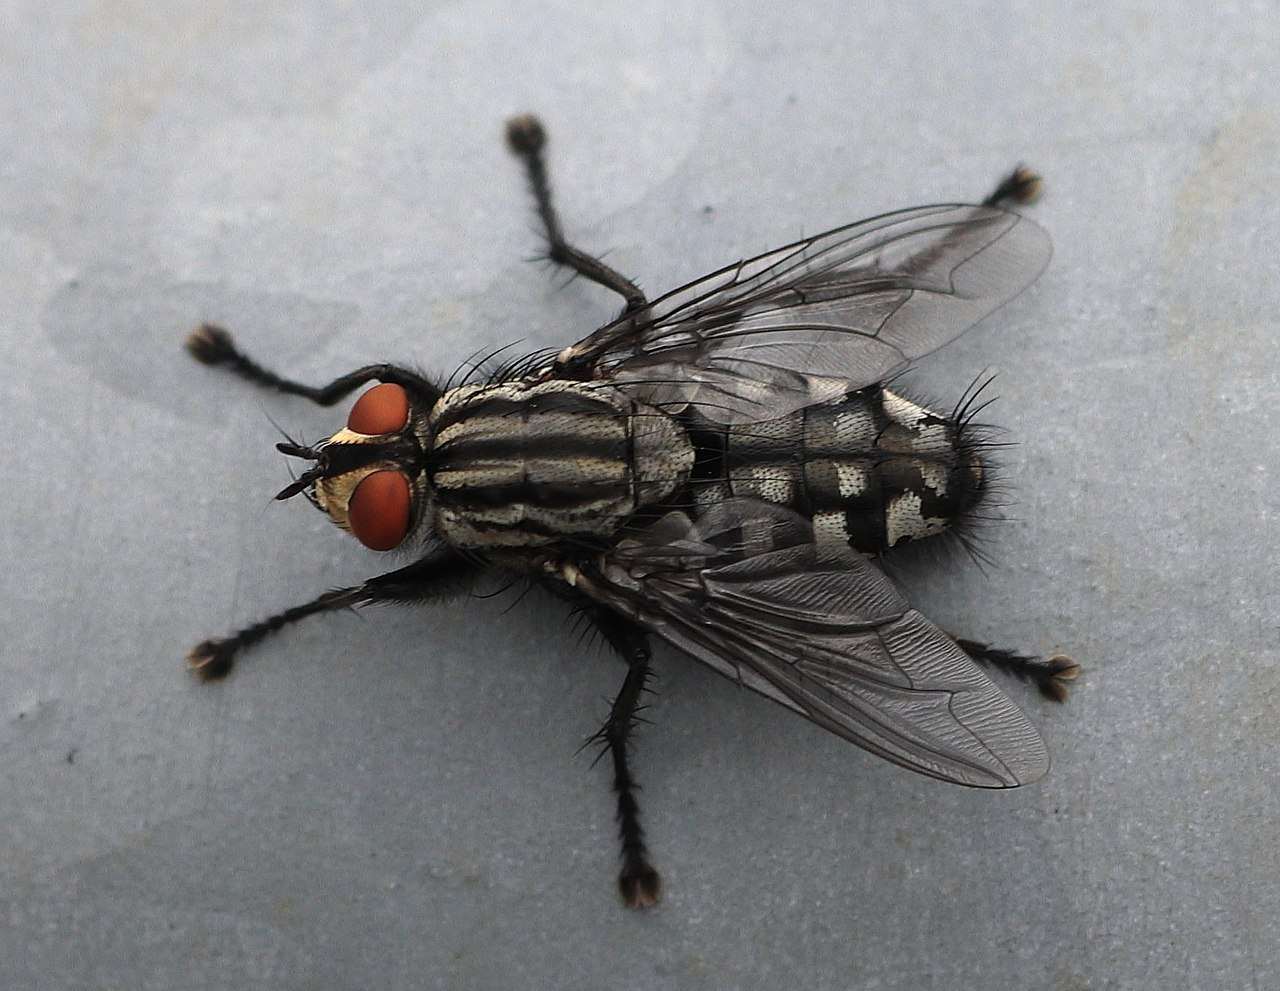
\includegraphics[height=4cm]{flesh-fly.jpg}
        \caption{A Flesh-fly}
        \label{fig:flesh-fly}
    \end{minipage}%
    \begin{minipage}{.5\textwidth}
        \centering
        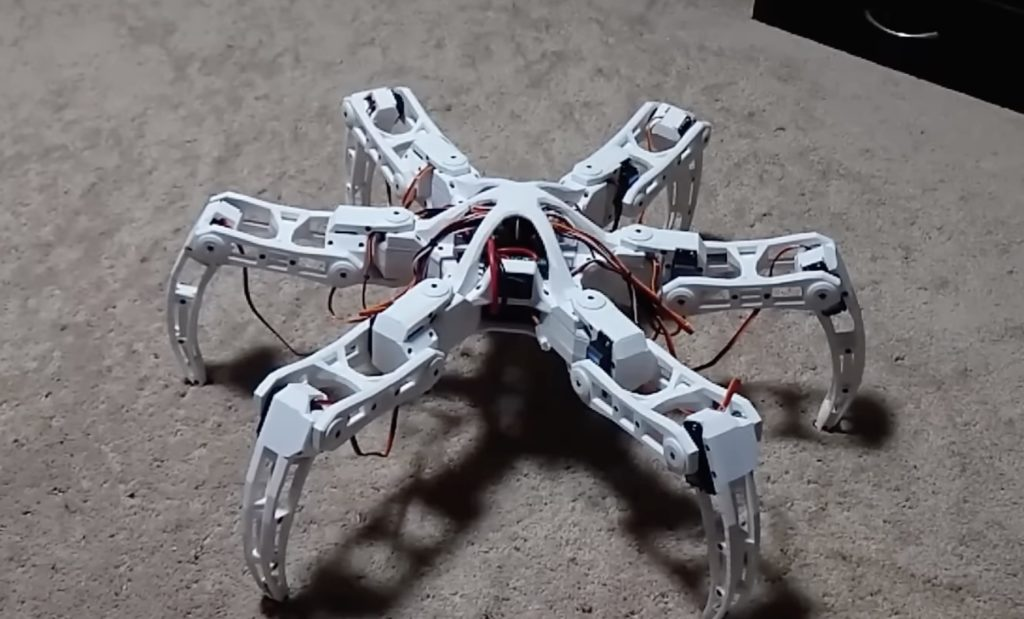
\includegraphics[height=4cm]{circ-hexapod.jpg}
        \caption{A circular hexapod}
        \label{fig:circ-hexapod}  
    \end{minipage}
\end{figure}

In the context of robotics "Hexapod" is used to refer to any robot with six legs, the most common configuration of Hexapods are either a rectangular
layout with three legs on either side mimicking biological Hexapoda, or a circular design with radially symmetrical leg spacing,
as seen in \autoref{fig:circ-hexapod}

The hexapod possess the minimum number of legs to allow a naturally stable platform since while taking a step there can be upwards of three anchor points around the center of mass at all times.
This makes the hexapod hexapods an ideal platform to navigate complex terrain while maintain stability, without requiring advanced balancing control systems.

For a hexapod to walk it must lift some of its legs while bracing with others, the number of swinging to bracing legs, and how each is moved, is referred to as the walking "gait".
The chosen gait influences the speed and stability of the hexapod, the tripod gait is considered to be the most well rounded, having good speed and stability.
In the tripod gait three legs are bracing while the remaining three swing. A example of a more stable gait would be the One by One gait, where only one leg is moved at a time.

It is also possible to create a system where there is no predetermined gait, but rather the system determines the optimal legs to brace and swing depending on the current walking environment.

\section{Control}
Walking over rough terrain requires a control system to correctly actuate the hexapods legs. Various types of control schemes exist, the primary schemes are traditional controllers,
bio-inspired controllers and \ac{rl}. These three schemes are discussed below. Control trends can be seen in \autoref{fig:control-trends}
\begin{figure}[h]
    \centering
    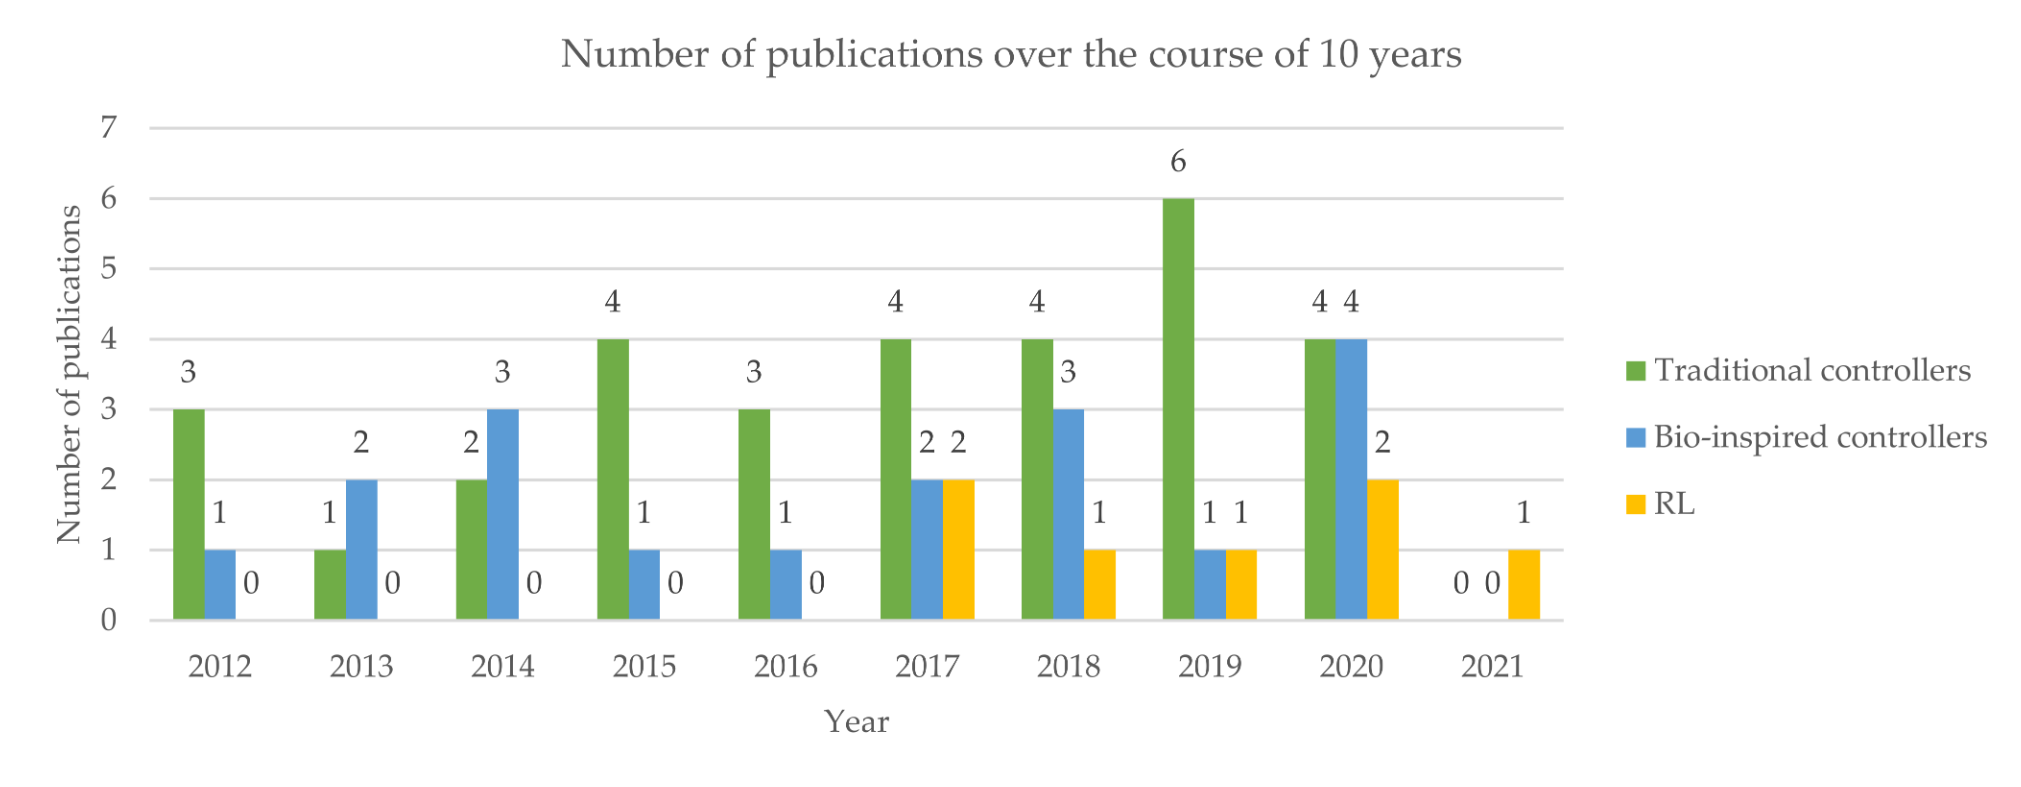
\includegraphics[width=\textwidth]{contoroller-trends.png}
    \caption{Trends of hexapod control schemes \citep{coelho2021trends}}
    \label{fig:control-trends}
\end{figure}

    \subsection{Traditional}
    Traditional controllers rely on an exact mathematical model of the robot and \ac{ik} to calculate angular commands for all leg joints. This method of control is purely kinematic does not 
    take into account external forces applied to the robot, thus it does not inherently adjust to the environment.

    Instead of a purley kinematic model, a dynamic model can also be used. Using a dynamic model the forces acting on the robots legs are taken into account, usually acquired through torque measurements 
    from servos. By taking applied torque into account dynamic model controllers will intrinsically detect a deviation when an external force is applied to the robot or its legs and compensate appropriately.

    It should be noted that it is possible for a kinematic model controller to also adjust to external disturbances, but this is not intrinsic to the control model and requires additional control logic.
    
    \subsection{Bio Inspired}
    Bio inspired controllers attempt to mimic the neural structure of animals to achieve the same locomotion methods that they use. This is implemented through the use of a \ac{ann}
    If implemented successfully a bio inspired controller can be highly adaptable to the surrounding environment and is even able to adapt to damaged or missing legs.

    \subsection{\acl{rl}}
    \ac{rl} controllers are created through using trial and error to construct a neural net that minimises a cost function for a specific goal. This theoretically allows \ac{rl} controllers to adapt to any
    circumstances given enough time, allowing a very hight level of autonomy, as no prior direction is required. \ac{rl} controllers are though notoriously difficult to train properly, especially when the 
    amount of sensors and control outputs grow large, increasing the feature space. And event he most well trained \ac{rl} agent still has the possibility to exhibit inexplicable behaviour.
    
\section{Sensors}
    No matter the control scheme used, to know where to place its feet the robot requires sensor(s) to sense its environment in some way, this could be achieved through simple sensors such as servo torque or touch,
    as used in \cite{t}. Or more advanced methods such as vision or \ac{lidar} could be used, as shown in \cite{t}.

    Depending on the terrain navigation system it might be required to localise the robot in 3D space, for this it is possible to use external sensors such as a type of beacon (RF, Reflective, Ultrasonic), \ac{gps}
    or, through the use of a \ac{slam} system, internal sensors, such as vision could be used.

    The 

    \subsection{End Effector Placement Method}

    Among other research focused on hexapods, many focus on topics such as obstacle avoidance, climbing surfaces, confined surfaces and cargo transportation.
    When focusing of terrain adaptation most often the use of sensors such as \ac{lidar}, torque, or touch are employed. Where usually the height of end effectors
    are adjusted to the height of the terrain \cite{coelho2021trends}.

    Some papers, such as \cite{homberger2017terrain} utilise stereoscopic vision, in addition to end effector height adjustment, also focus on surface material classifications based on which the virtual
    stiffness of the impedance controller is adjusted.

    The focus of this paper will be on end effector height and planar position adaptation through real time walkability classification of the environment. 
    While only utilising an \ac{rgbd} camera as sensor

    \subsection{Localisation and Mapping}

    This project requires a system that will localise the robot within its environment, as the primary sensor used is an \ac{rgbd} camera various visual \ac{slam} systems 
    were considered. ORB-SLAM 3, a optimisation-based, sparse map \ac{slam} system was chosen to be used. ORB-SLAM 3 maintains a sparse map, an atlas, of both active and
    dormant features. This atlas is used to localise in the sparse map \citep{macario2022comprehensive}.

    The implementation of a dense map to be used for end effector placement is discussed in \autoref{chap:mapping}.

\section{Simulation Environment}

The most popular physics simulators for robotics in recent times are Gazebo, \ac{mujoco} and CoppeliaSim (previously V-REP) \citep{Collins-2021}.
Gazebo and CoppeliaSim both have easy to use \ac{gui} interfaces and easy integration with \ac{ros}. \ac{mujoco} on the other hand does not have
a full \ac{gui} interface, only a simulation viewer, and does not have native \ac{ros} integration. Having said this \ac{mujoco} was found to be
the most accurate and fastest simulator when considering the use case of robotics \citep{Erez-2015}.

Considering that the only relevant downside to \ac{mujoco} is the lack of native \ac{ros} integration and the lack of a comprehensive \ac{gui},
which seeing as \ac{mujoco} has good python bindings, could be seen as a advantage, \ac{mujoco} was chosen as the simulator.

\chapter{Content chapter}

Unless the chapter heading already makes it clear, an introductory paragraph that explains how this chapter contributes to the objectives of the report/project.

\section{Heading level 2}

\subsection{Heading level 3}

\subsubsection{Deepest heading, only if you cannot do without it}
\vspace{2cm}

\paragraph{Equations:}

An equation must read like part of the text. The solution of the quadratic equation $ax^2+bx+c=0$ given by the following expression (note the full stop after the equation to indicate the end of the sentence):
\begin{equation}
    x = \frac{-b \pm \sqrt{b^2-4ac}}{2b} .
\end{equation}
In other cases the equation is in the middle of the sentence. Then the paragraph following the equation should start with a small letter. Euler's identity is 
\begin{equation}
    e^{i \pi} + 1 = 0 ,
\end{equation}
where $e$ is Euler's number, the base of natural logarithms.

The \texttt{amsmath} has a wealth of structure and information on formatting of mathematical equations.

\pagebreak
\paragraph{Symbols and numbers:}

Symbols that represent values of properties should be printed in italics, but SI units and names of functions (e.g. sin, cos and tan) must not be printed in italics. There must be a small hard space between a number and its unit, e.g. \qty{120}{km}. Use the \texttt{siunitx} package to typeset numbers, angles and quantities with units:
\begin{tabbing}
\hspace*{\parindent}\=\verb|\qty{20}{N.m}|\quad\=$\rightarrow$\quad\=\kill
    \>\verb|\num{1.23e3}| \>$\rightarrow$\> $\num{1.23e3}$ \\
    \>\verb|\ang{30}|     \>$\rightarrow$\> $\ang{30}$ \\
    \>\verb|\qty{20}{N.m}|\>$\rightarrow$\> $\qty{20}{N.m}$
\end{tabbing}

\paragraph{Figures and tables:}
The \texttt{graphicx} package can import \texttt{PDF}, \texttt{PNG} and \texttt{JPG} graphic files.

\begin{table}[htbp]
    \centering
    \caption{Standard ISO paper sizes}
    \label{tab:paper}
    \begin{tabular}{lcccc}
    \hline
        Paper\quad && \multicolumn{3}{c}{Sizes} \\
    \cline{2-5}
        &&  $W$      && $H$ \\
        && \small [mm] &&  \small [mm]   \\
    \cline{1-1}\cline{3-3}\cline{5-5}
        A0 && 841 && 1189 \\
        A1 && 594 &&  841 \\
        A2 && 420 &&  594 \\
        A3 && 297 &&  420 \\
        A4 && 210 &&  297 \\
        A5 && 148 &&  210 \\
    \hline
    \end{tabular}
\end{table}


\begin{figure}[htbp]
    \centering
    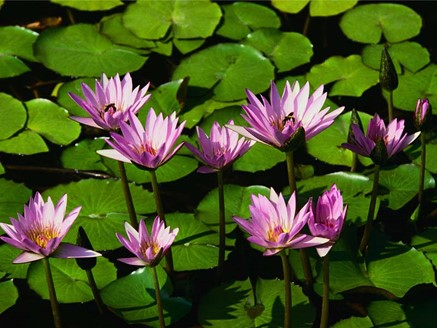
\includegraphics[scale=0.75]{figs/waterplants}
    \caption{Water plants}
    \label{fig:waterplant}
\end{figure}

\chapter{Conclusions}


\appendix%------------------------------------------------------------
\chapter{Mathematical proofs}

\section{Euler's equation}
Euler's equation gives the relationship between the trigonometric functions and the complex exponential function.
\begin{equation}
    e^{ i\theta } = \cos \theta + i\sin \theta
    \label{eq:Euler}
\end{equation}
Inserting $\theta=\pi$ in \eqref{eq:Euler} results in Euler's identity
\begin{equation}
    e^{ i \pi} + 1 = 0
    \label{eq:Euler2}
\end{equation}


\section{Navier Stokes equation}

The Navier–Stokes equations mathematically express momentum balance and conservation of mass for Newtonian fluids.  Navier-Stokes equations using tensor notation:
\begin{subequations}
\begin{gather}
    \frac{\partial \rho}{\partial t} +
    \frac{\partial}{\partial x_j}\left[ \rho u_j \right] = 0 
    \\
    \frac{\partial}{\partial t}\left( \rho u_i \right) +
    \frac{\partial}{\partial x_j}
    \left[ \rho u_i u_j + p \delta_{ij} - \tau_{ji} \right] = 0, \quad i=1,2,3
    \\
    \frac{\partial}{\partial t}\left( \rho e_0 \right) +
    \frac{\partial}{\partial x_j}
    \left[ \rho u_j e_0 + u_j p + q_j - u_i \tau_{ij} \right] = 0
\end{gather}
\end{subequations}

\chapter{Experimental results}


\backmatter%----------------------------------------------------------
\bibliography{bib/bib-sample}
 
\end{document}   

